Quando tratamos destes sistemas no ensemble canônico a energia interna não mais será minimizada no nosso sistema termalizado. Introduzimos uma nova grandeza chamada Energia Livre de Helmholtz ($F$), definida como a transformada de Legendre (discutida no Apêndice \ref{apdx: legendre}) da energia interna em relação à entropia, ou seja

\begin{equation}
	U(S,V,N) \mapsto F(T, V, N)
\end{equation}

ou ainda mais especificamente

\[
F(T, V, N) = U(S(T,V,N), V, N) - T S(T,V,N) 
\]

Note ainda as diferenciais

\begin{align*}
	& dU = TdS - PdV + \mu dN \\
	& dF = -SdT - PdV + \mu dN
\end{align*}

Para o desenvolvimento da função partição estamos atentos aos requisitos do ensemble canônico. Um sistema termalizado por um banho térmico. Nosso sistema completo pode ser representado

\begin{center}
	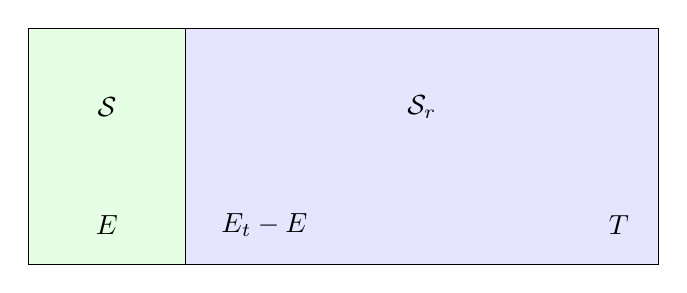
\begin{tikzpicture}
		\fill[blue!10!white] (0,0) rectangle (8,3);
		\draw (0,0) rectangle (8,3);
		\fill[green!10!white] (0,0) rectangle (2,3);
		\draw (0,0) rectangle (2,3);
		\node at (1,2) {$\mathcal{S}$};
		\node at (1,0.5) {$E$};
		\node at (5,2) {$\mathcal{S}_r$};
		\node at (7.5,0.5) {$T$};
		\node at (3,0.5) {$E_t - E$};
	\end{tikzpicture}
\end{center}

Considere que os sistemas estão em contato térmico e o sistema completo, junto com o banho é um sistema isolado de energia $E_t$. Sabemos que a probabilidade de uma energia no nosso sistema termalizado ($\rho_E$) é expressa:

\[
\rho_E = \sum_{\sigma} \rho_\sigma = \Omega(E)\rho_\sigma
\]

Onde note, $\rho_\sigma$ é a probabilidade de, dada uma temperatura, um microestado possível. Note por outro lado que podemos expressar:

\[
\rho_E = \frac{\Omega(E) \Omega_r (E_t - E)}{\sum_{i} \Omega(E_i) \Omega_r(E_t-E)}
\]

Note que isso é nada mais do que dizer que os microestados são equiprováveis e basta uma contagem (normalizada) para definir a probabilidade. Neste sentido podemos também escrever:

\[
\rho_\sigma \propto \Omega_r(E_t - E)
\]

Isso é, quanto mais formas o reservatório possa se organizar para determinada energia, mais provável é o microestado associado à energia de $\mathcal{S}$.

\begin{align*}
	\rho_\sigma & \propto e^{\beta T K_b \log{(\Omega_r(E_t - E))}} \\
	& \propto e^{\beta T \left( \mathcal{S}_r(E_t) - \frac{E}{T}\right) } \\
	& \propto e^{-\beta E} e^{\beta T \mathcal{S}_r(E_t)} \\
	& \propto e^{-\beta E}
\end{align*}

Onde fizemos a expansão de $k_b \log{(\Omega_r(E_t - E))}$ (entropia) em Taylor (apesar de que, em realidade, apenas $\frac{E}{E_t}$ é pequeno, não necessariamente $E$) e obtivemos

\[
\mathcal{S}_r(E_t - E) \approx \mathcal{S}_r(E_t) + \left( \frac{\partial \mathcal{S}_r}{\partial E}\right)_{E=E_t} (-E)
\]

Onde 

\[
\left( \frac{\partial \mathcal{S}_r}{\partial E} \right)_{E=E_t} = \frac{1}{T}
\]

Um sistema termalizado vai querer minimizar essa nova grandeza da energia livre de Helmholtz. Em todo caso iniciaremos com a expressão já deduzida da equação de partição

\[
\mathcal{Z} = \sum_{\sigma} e^{-\beta E_\sigma}
\]

Que pode ser reescrito em termos de uma soma na energia

\begin{align*}
	& \mathcal{Z} = \sum_{E} e^{-\beta E} \Omega(E) \\
	& \mathcal{Z} = \sum_{E} e^{-\beta T K_b \log{(\Omega(E))}} \Omega(E)
\end{align*}

Podemos argumentar que $ K_b \log{(\Omega(E))} = S(E)$ e usaremos o logaritmo de somas assintóticas (discutido no Apêndice \ref{apdx: somaassin}) para terminar o desenvolvimento. Note

\begin{align*}
	& \log{(\mathcal{Z})} \approx \log{\left( \max_x{[e^{-\beta(E - T S(E))}]} \right)} \\
	& \log{(\mathcal{Z})} \approx \log{\left(e^{-\beta \min_E{((E - T S(E)))}} \right)}
\end{align*}

Onde podemos reconhecer pela transformada de Legendre o termo referente à Energia livre de Helmholtz. Tendo assim

\[
\log{(\mathcal{Z})} \approx -\beta F
\]	

\begin{equation}
	F = - K_b T \log{(\mathcal{Z})}
\end{equation}
